An op amp designed to have a low-frequency gain of $10^{5}$ and a high-frequency response dominated by a single pole at 100 rad/s, acquires, through a manufacturing error, a pair of additional poles at 10,000 rad/s. 
\begin{enumerate}
\item At what frequency does the total phase shift reach 180$\degree$ ? 
\item At this frequency, for what value of $\beta$, assumed to be frequency independent, does the loop gain reach a value of unity? 
\item What is the corresponding value of closed-loop gain at low frequencies?
\end{enumerate}
%\begin{enumerate}[label=\thesection.\arabic*.,ref=\thesection.\theenumi]
\begin{enumerate}[label=\arabic*.,ref=\theenumi]
\numberwithin{equation}{enumi}
\item Find $G(s)$
\solution
\begin{align}
G(s) &= \frac{A}{1+\frac{s}{p}} 
\end{align}
Considering manufacturing error
\begin{align}
G(s) &= \dfrac{A}{(1+\dfrac{s}{p})(1+\dfrac{s}{p_{error}})} 
\\
A &= \text{Low Frequency Gain} = 10^{5}
\\
p &= 100
\\
p_{error} &= 10^{4}
\\
G(s) &= \dfrac{10^{5}}{(1+\dfrac{s}{100})(1+\dfrac{s}{10^{4}})^{2}}
\\
\measuredangle G(j\omega) &= -\tan^{-1}\frac{\omega}{100} - 2\tan^{-1}\frac{\omega}{10^{4}}
\end{align}
\item Calculating the frequency at which the total phase shift reach 180$\degree$ 

At $\omega_{180}, \measuredangle G(j\omega_{180}) = -180\degree$

Also $\omega_{180} >> 100$
\begin{align}
180\degree &= 90\degree  + 2 \tan^{-1}(\frac{\omega_{180}}{10^{4}})
\\
\tan^{-1}\frac{\omega_{180}}{10^{4}}&= 45\degree
\\
\frac{\omega_{180}}{10^{4}} &= \tan 45\degree = 1
\\
\omega_{180} &= 10^{4} rad/s
\end{align}
\begin{figure}[!ht]
\centering
    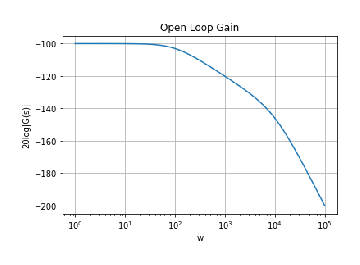
\includegraphics[width=\columnwidth]{./figs/ee18btech11001/Figure_1.eps}
  \caption{Open Loop Gain}
  \label{fig:ee18btech11001_fig1}
\end{figure}
\item Calculating feedback factor $\beta$ for which loop gain at $\omega_{180}$ is unity
\begin{align}
H(s) = G(s)\beta = 1
\\
\dfrac{10^{5}\beta}{\sqrt{1^{2} + (\dfrac{\omega_{180}}{10^{2}})^{2}} \sqrt{(1+\dfrac{\omega_{180}}{10^{4}})^{2}}} = 1
\\
\beta = 0.002
\end{align}
\item Calculating the closed loop gain at low frequency
Let $T(s)$ be the closed loop Transfer Function.
\begin{figure}[!hbt]
	\begin{center}
			\resizebox{\columnwidth}{!}{\begin{circuitikz}[american ]
\draw (0,0) to [R,l_=$R_{E1}$](0,-2) to node[ground]{}++(0,-0.25) ++(6,0)
(0,0) to [R,l_=$R_F$](3,0) to [R,l_=$R_{E2}$]++(0,-2)to node[ground]{}++(0,0)
(3,0)--(5,0)to [current source,l_=$-I_o$]++(0,-2) to node[ground]{}++(0,-0.5)
(0,0)--(-2,0) to [open, v^>=${V}_f$,*-] ++(0,-1) ++(6,0)
(0,0) 
;\end{circuitikz}
}
	\end{center}
\caption{Closed loop circuit}
\label{fig:equivalent_system}
\end{figure}

\begin{align}
T(s) &= \dfrac{G(s)}{1+\beta G(s)}
\\
T(s) &= \dfrac{10^{5}}{1+\beta 10^{5}+ \dfrac{s}{100}}
\end{align}

\begin{align}
|T(s)| &= \dfrac{10^{5}}{\sqrt{(200)^{2} + (\frac{s}{100})^{2}}}
\end{align}
At low frequencies
\begin{align}
|T(s)| &= 500 V/V
\end{align}

\begin{table}[!ht]
\centering
\input{./tables/ee18btech11001/table1.tex}
\caption{Obtained Parameters}
\label{table:ee18btech11001_params}
\end{table}


\begin{figure}[!ht]
\centering
    \includegraphics[width=\columnwidth]{./figs/ee18btech11001/Figure_2.eps}
  \caption{Closed Loop Gain}
  \label{fig:ee18btech11001_fig2}
\end{figure}

\begin{figure}[!ht]
\centering
    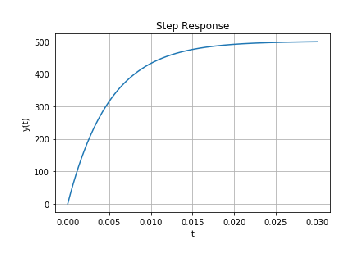
\includegraphics[width=\columnwidth]{./figs/ee18btech11001/Figure_3.eps}
  \caption{Step Response}
  \label{fig:ee18btech11001_fig3}
\end{figure}
The following code performs all the calculations of above equations
\begin{lstlisting}
codes/ee18btech11001/code1.py
\end{lstlisting}

The following code plots the open loop gains, closed loop gains and step response to the system
\begin{lstlisting}
codes/ee18btech11001/code2.py
\end{lstlisting}


\item Designing the circuit for transfer function $G(s)$
\begin{figure}[!hbt]
	\begin{center}
			\resizebox{\columnwidth}{!}{\begin{circuitikz}
\ctikzset{bipoles/length=1cm}
\draw
(0, 0) node[op amp] (opamp) {}
(opamp.-) to[R,l_=$R_1$,-o] (-2, 0.35) -- (-3, 0.35) {}
(opamp.-) to[short,*-] ++(0,0.5) coordinate (leftC)
to[R=$R_2$] (leftC -| opamp.out)
to[short,-*] (opamp.out) to [short,-o] (1.5,0)
(opamp.+) -- (-1,-0.35) to (-1,-0.5) node[ground]{}
(opamp.-) to[short,*-] ++(0,1.5) coordinate (leftC)
to[C=$C_1$] (leftC -| opamp.out) to[short,-*] (opamp.out)

node at (-2.5,0.6){$V_{in}$}
node at (0.45,-5){$V_{out}$}
node at (-1.1,1.8){$V_{1}$}
node at (-1.9,-6.15){$V_{3}$}
node at (0.8 , -1.15){$V_{2}$}
node at (1.5,0.25) {$V_{o1}$}
node at (-3,-1.05) {$V_{o2}$}
;

\draw 
(0,-3.5) node[op amp ,xscale = -1] (opamp2) {}
(1.5,0) to [R,l_=$R_3$,-o] (1.5, -3.15) to (opamp2.-)
(opamp2.+) to[short,*-] (1.5,-3.85) to (1.5,-4.2) node[ground]{}
(opamp2.-) to [short,*-] (0.8,-2.85) to [R,l_=$R_4$,-o] (-1.5,-2.85)
(0.8,-2.85) to [short,*-] (0.8,-1.45) to [C,l=$C_2$,-o] (-1.5 , -1.45)
(opamp2.out)to [short,*-](-1.5,-3.5) to [short,*-](-1.5 , -1.45) to [short,*-](-1.5 , -2.45)
;

\draw 
(-1.5 , -1.45) to [short,*-] (-3,-1.45) to [short,*-] (-3,-5.7)
(-1,-5.35) node[op amp,yscale=-1] (opamp3) {}
(-3,-5.7) to[R,l_=$R_3$,-o] (-2, -5.7) to [short,-*] (opamp3.-)
(opamp3.-) to [short,*-] (-1.85,-7.5) to [R,l_=$R_4$,-o] (0.25,-7.5)
(-1.85,-6.5) to [C,l_=$C_2$,-o] (0.25,-6.5)
(opamp3.out) to [short,*-] (0.25,-5.35) to [short,*-] (0.25,-6.5) to [short,*-] (0.25,-7.5)
(opamp3.+) to [short,*-] (-1.85,-4) to [short,*-] (-2.5,-4) to (-2.5,-4.6) node[ground]{}

;


\end{circuitikz}}
	\end{center}
\caption{1}
\label{fig:equivalent_system1}
\end{figure}

Let us assume Op-Amp to be ideal. So this means $V_{1}=0$
Applying KCL at node $V_{1}$

\begin{align}
I_{in} &= I_{C_{1}} + I_{R_{2}}
\\
\dfrac{V_{in}}{R_{1}} &= \dfrac{V_{out}}{R_{2}} + C_{1}\dfrac{dV_{out}}{dt}
\end{align}
In Laplace domain
\begin{align}
\dfrac{V_{in}(s)}{R_{1}} &= \dfrac{V_{out}(s)}{R_{2}} + C_{1}sV_{out}(s)
\\
\dfrac{V_{out}}{V_{in}} &= \dfrac{R_{2}/R_{1}}{1+sR_{2}C_{1}}
\\
T(s) &= \dfrac{10^{5}}{1+\frac{s}{100}}
\\
\frac{R_{2}}{R_{1}} &= 10^{5}
\\
R_{2}C_{1} &= \frac{1}{100}
\end{align}


\begin{table}[!ht]
\centering
\input{./tables/ee18btech11001/table2.tex}
\caption{Circuit Parameters}
\label{table:ee18btech11001_params2}
\end{table}

\item Verification of circuit design through SPICE

\begin{figure}[!ht]
\centering
    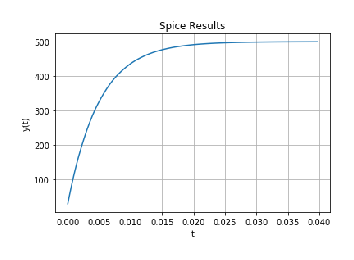
\includegraphics[width=\columnwidth]{./figs/ee18btech11001/Figure_4.eps}
  \caption{SPICE simulation of circuit \ref{fig:equivalent_system1}}
  \label{fig:ee18btech11001_fig5}
\end{figure}

A SPICE simulation of circuit \ref{fig:equivalent_system1} is done by providing a DC input(Unit Step Input). The obtained plot (figure \ref{fig:ee18btech11001_fig5}) is similar to the Step response of the feedback system in figure \ref{fig:ee18btech11001_fig3}. Hence we verify our design is correct.



The following code plots the SPICE simulation results
from SPICE plot txt file

\begin{lstlisting}
codes/ee18btech11001/spice/plotter.py
\end{lstlisting}
\end{enumerate}
